\documentclass[11pt, oneside]{article}   	% use "amsart" instead of "article" for AMSLaTeX format


% \usepackage{draftwatermark}
% \SetWatermarkText{Draft}
% \SetWatermarkScale{5}
% \SetWatermarkLightness {0.9} 
% \SetWatermarkColor[rgb]{0.7,0,0}


\usepackage{geometry}                		% See geometry.pdf to learn the layout options. There are lots.
\geometry{letterpaper}                   		% ... or a4paper or a5paper or ... 
%\geometry{landscape}                		% Activate for for rotated page geometry
%\usepackage[parfill]{parskip}    		% Activate to begin paragraphs with an empty line rather than an indent
\usepackage{graphicx}				% Use pdf, png, jpg, or eps� with pdflatex; use eps in DVI mode
								% TeX will automatically convert eps --> pdf in pdflat						
								% TeX will automatically convert eps --> pdf in pdflatex		
\usepackage{amssymb}
\usepackage{amsmath}
\usepackage{amsthm}
\usepackage{mathrsfs}
\usepackage{hyperref}
\usepackage{url}
\usepackage{subcaption}
\usepackage{authblk}
\usepackage{mathtools}
\usepackage{graphicx}
\usepackage[export]{adjustbox}
\usepackage{fixltx2e}
\usepackage{hyperref}
\usepackage{alltt}
\usepackage{color}
\usepackage[utf8]{inputenc}
\usepackage[english]{babel}
\usepackage{float}
\usepackage{bigints}
\usepackage{braket}
\usepackage{siunitx}

\theoremstyle{definition}
\newtheorem{thm}{Theorem}[section]
% \newtheorem{defn}[thm]{Definition}
\newtheorem{definition}{Definition}[section]
\newtheorem{example}{Example}[section]
% \newtheorem[thm]{exmp}
\newtheorem{proposition}{Proposition}[section]

\newtheorem{question}{Question}[section]



\newcommand{\veq}{\mathrel{\rotatebox{90}{$=$}}}
\DeclareMathOperator{\bda}{\Big \downarrow}

\DeclareMathOperator{\mymod}{\text{mod}}

\DeclareMathOperator{\E}{\mathbb{E}}
\newcommand{\argmax}{\operatornamewithlimits{argmax}}
\newcommand{\argmin}{\operatornamewithlimits{argmin}}


\title{A Few Notes on Capital Gains Taxation in Trusts}
\author{David Meyer \\ dmm@\{1-4-5.net,uoregon.edu\}}

\date{Last update: \today}							% Activate to display a given date or no date



\begin{document}
\maketitle

\section{Introduction}

This document started life as research I did after discussing taxation issues with Denise on 07-May-2019. There was also a confusing email thread with amy@windes.com but 
I have completely abandoned that as I couldn't make sense of what she said.

\bigskip
\noindent
This document is intended to answer the narrow question: 

\bigskip
\noindent
\begin{center}
\emph{What are the tax implications of "taking money out" of either trust?} 
\end{center}

\bigskip
\noindent
The exact meaning of "taking money out" discussed in Section \ref{sec:tmo}.

\bigskip
\noindent
As an aside, remember that there are two main kinds of trusts: simple and complex. In our case, the Non-Exempt trust is a simple trust while the Exempt trust is a complex trust.
Simple and complex trusts have a many different features. 
For example, a simple trust is required to distribute all  \emph{income} to the beneficiaries who then pay tax at their personal rate.  On the other hand, a 
complex trust such as the Exempt trust is \emph{not required} to distribute its income; however, if it holds income for more than one year then it pays tax at the trust income 
tax rate; see Section \ref{sec:taxation_in_trust}.  

\bigskip
\noindent
One other trust property that will be useful in reading the tax tables later: grantor vs. non-grantor trusts. What we need to know here is that our trusts are
are non-grantor trusts.


\bigskip
\noindent
Finally, standard disclaimer: I learned everything in this document myself by studying what I could find. 

\bigskip
\noindent
The remainder of this document is organized as follows: Section \ref{sec:trust_terminology_and_concepts} briefly reviews trust terminology and concepts that we need for 
this discussion. Section \ref{sec:tmo} examines what "taking money out" means and what process might be used to do so. Section \ref{sec:taxation_in_trust} discusses
how taxation works in the trust context, focusing narrowly on capital gains taxes. Section \ref{sec:examples} provides a few worked examples and 
Section \ref{sec:open_questions} lists a few open questions.





\section{Brief Review: Trust Terminology and Concepts}
\label{sec:trust_terminology_and_concepts}
In this section I'll try to define a few terms and concepts just to be sure we're all on the same page

\bigskip
\noindent
First, and most importantly, trusts, like estates, are taxable entities. A trust is a fiduciary entity whose objective is to hold and 
invest money or property held in the trust for the benefit of the beneficiaries. Trust property
consists of \textbf{principal} (aka \textbf{corpus}), which is the property transferred
to the trust by the grantor, and income earned by the trust, usually
from investments\footnote{You can think of the principal as what was there when you received the trust, although like everything with trusts, not exactly.} 

\bigskip
\noindent
If the trust retains \emph{income} beyond the end of the calendar year, then it must pay taxes on it at the trust tax rate; see
Section \ref{sec:taxation_in_trust}.  If money is distributed to the beneficiaries, then whether it is taxable or not to the
beneficiaries will depend on whether principal or income was distributed, and if it was income, then whether it was tax-free income 
or retained income from previous years that the trust has already paid tax on. In our case so far everything distributed
from both trusts has been income which is taxed at the beneficiary's rate, not the trust rate.

\subsection{Income Tax. vs. Capital Gains Tax: A Quick Overview}
\textbf{Income tax} is paid on earnings from interest, dividends, employment,
royalties, or self-employment, whether it's in the form of services,
money, or property. 

\bigskip
\noindent
\textbf{Capital gains tax} is paid on income that derives
from the sale or exchange of an asset, such as a stock or property
that's categorized as a capital asset. 

\bigskip
\noindent
Of course there are many other kinds of tax, but income and capital gains are the taxes we are interested in for our 
purposes here.

\subsection{What can be distributed tax-free to the beneficiaries?}

\bigskip
\noindent
Because trusts are not subject to double taxation, either principal or income on which the trust paid taxes can be distributed
tax-free to the beneficiaries. Likewise, any taxable distribution to beneficiaries is deductible by the trust. You can think of this
like this: either the trust pays tax or the beneficiary pays tax, but not both. 

\bigskip
\noindent
There is an interesting point to note here: Because there is no double taxation and because it is assumed that tax has been paid
on the principal (there is an open question with this,  see Section \ref{sec:open_questions}), principal can apparently be distributed \textbf{tax-free} to 
the beneficiaries if the trust allows this. Of course if there are any capital gains you will have to pay tax on that. This is discussed 
in both Sections \ref{sec:taxation_in_trust} and \ref{sec:examples}.

\bigskip
\noindent
\textbf{Denise:} This answers one of your questions. If the trust has stock in XYZ corporation and the cost basis is the same
as the sale price, then the  proceeds of the sale can be distributed to the beneficiary (you) \textbf{tax-free} (as it is 
assumed that any principal has already been taxed and the trusts are non-double taxxation). So in your example if your cost 
basis on XYZ is 10.00 and the current price of XYZ shares is 10.00, then the trust's capital gain are zero and it can distribute 
all of the proceeds of the sale to you  tax free. At least that is what it looks like.




\section{"Taking Money Out" -- What exactly does this mean?}
\label{sec:tmo}
Denise and I discussed this for a while and it turns out that "taking money out" really means liquidating some asset (in our case 
stocks, bonds, ETFs or mutual funds, anything that is in WFA), paying the capital gains (if any), and having the proceeds distributed 
to the beneficiary. 

\bigskip
\noindent
I imagine this process would look something like the following. To be concrete, I'll use Denise as the beneficiary and Dan as the trustee.
Essentially this is the "taking money out" process.

\begin{enumerate}
\item Denise communicates to Dan that she wan't to liquidate some part of the trust principal to receive $X$ dollars
\item Dan, Denise and Dennis Dummit (I assume) figure out what to sell
\item Dennis makes the sale with proceeds $Y$
\item Someone (Dan?) computes the capital gains tax on the sale, call that $Z$
\item The trust distributes $Y - Z$ dollars to Denise, \textbf{tax free}. Ideally $X = Y - Z$.
\end{enumerate}

\bigskip
\noindent
Of course there will be fees from Wells Fargo and perhaps other expenses so we won't have exactly $X = Y - Z$.

\bigskip
\noindent
Now, the question remains: How to calculate Z, the capital gains tax. That is the subject of the next section.

\section{Overview: Taxation in Trusts}
\label{sec:taxation_in_trust}
First,  for income earned by the trust and not distributed, the trust (not the beneficiary) pays tax at the rate show in 
the row labeled "Estates and Non-Grantor Trusts" in Figure \ref{fig:2019_income_tax_schedule}. As you can see the 
top rate is 37\% on income greater \$12,750.00 (not 12,000, as Amy said). The thing to notice is the last column: 
the trust tax rate grows much faster than individual (or married, etc) rates do. For example, for Married Filing Jointly
you don't hit the top bracket of 37\% until \$612,350.00 (as opposed to  \$12,750.00 for the trust). In any event 
none of this comes into play for the capital gains case we are considering here.

\begin{figure}
\center{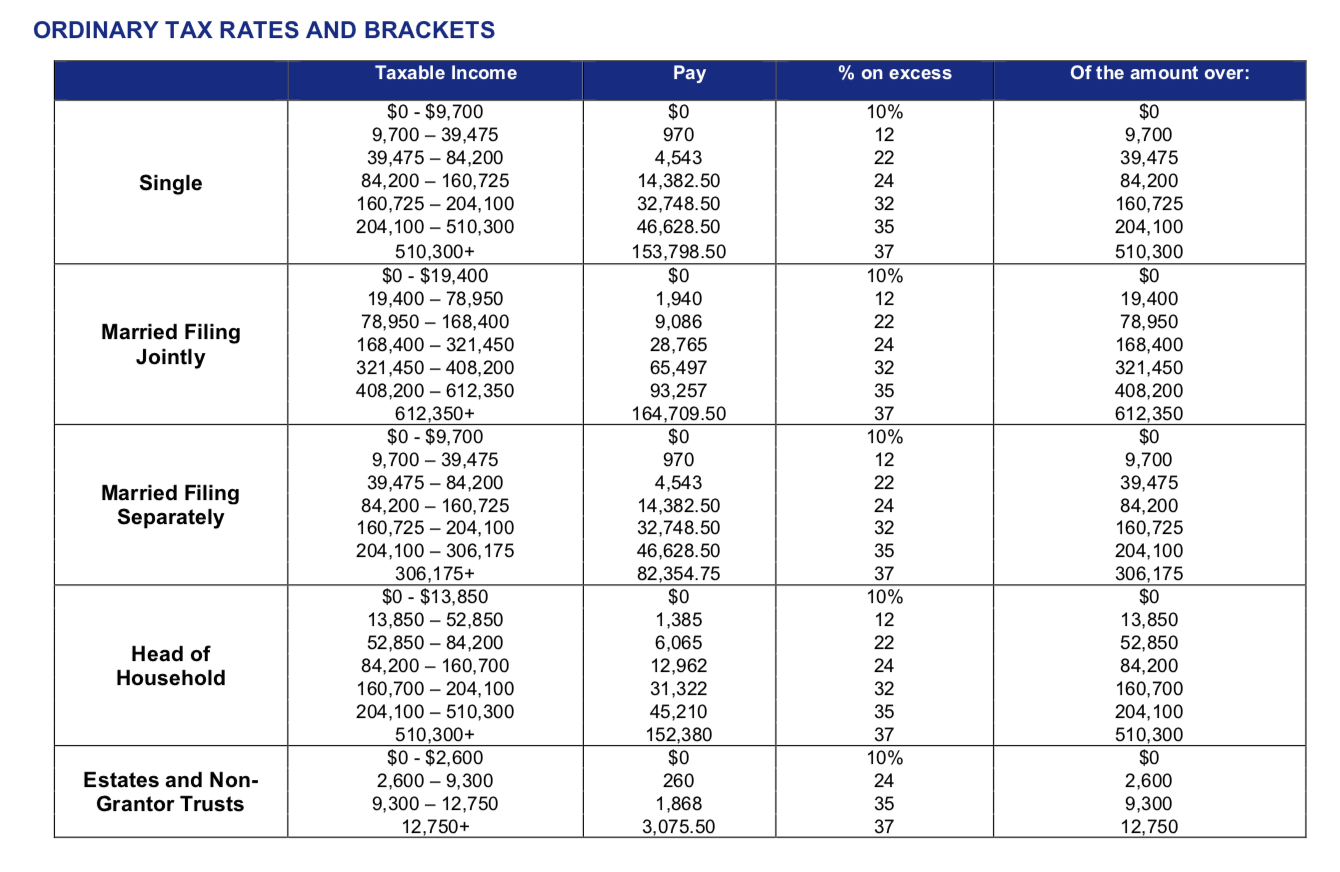
\includegraphics[scale=0.65] {images/2019_income_tax_schedule.png}}
\caption{2019 Income Tax Schedule (table courtesy Baird \cite{baird2019})}
\label{fig:2019_income_tax_schedule}
\end{figure}

\bigskip
\noindent
\textbf{Denise:} A lot of the confusion with Amy came from her apparent confusion over what your personal 
tax rates are and what the trust tax rates are. She seemed to be using of the word "your" to describe both your
FBO trust and your personal tax situation. In any event that confused most of what she said.

\bigskip
\noindent
Next, consider the capital gains case. The tax schedule is shown in Figure \ref{fig:2019_capital_gains_schedule}.
Here you can see that the maximum tax rate of 20\% for non-grantor trusts cuts in at capital gains above \$12,950.00. 
Again the rate increases much faster for trusts than it does for the other categories. 

\subsection{How To Calculate Capital Gains Tax}
First, every asset in the trust principal has a cost basis. The cost basis is essentially
what you (well, Dad) originally paid for the asset.\footnote{I think the cost basis was reset when we received the trusts, but not sure.}
So calculating the capital gains tax is pretty simple:
\begin{enumerate}
\item Calculate the capital gains
\item Apply the rate show in Figure \ref{fig:2019_capital_gains_schedule}
\end{enumerate}

\bigskip
\noindent
All this will become clearer if we look at a couple of examples.


\begin{figure}
\center{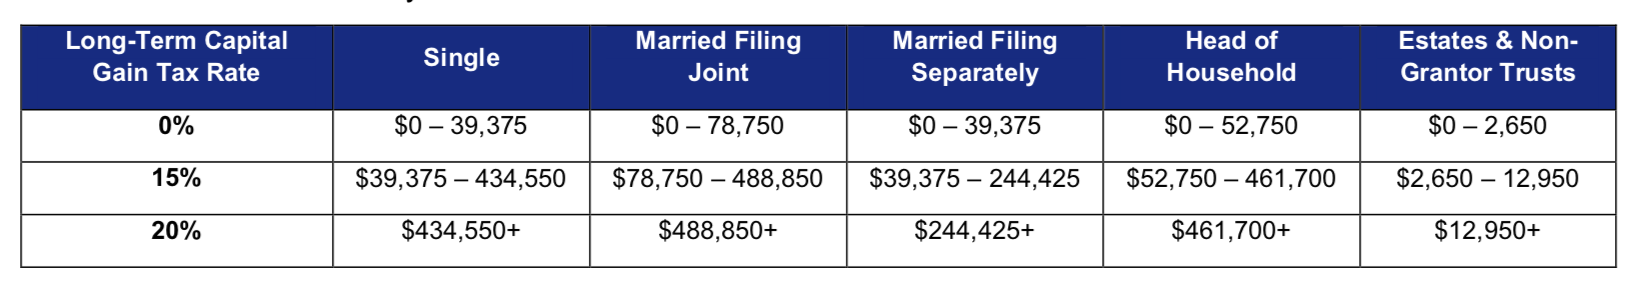
\includegraphics[scale=0.60] {images/2019_capital_gains_schedule.png}}
\caption{2019 Capital Gains Schedule (table courtesy Baird \cite{baird2019})}
\label{fig:2019_capital_gains_schedule}
\end{figure}

\section{Examples}
\label{sec:examples}
\textbf{Example 1:}  Suppose we want to "take out" \$100,000.00 from one of the trusts and we choose to have the trust sell shares of XYZ corporation
to accomplish this. Say XYZ shares are trading at \$10.00/share so the trust needs to sell 10,000 shares ($10,000 =  \frac{100,000.00}{10.00}$).
Suppose further that the trust's  cost basis on XYZ shares is \$5.00 so that the trust's \emph{capital gains} per share is $10.00 - 5.00 = 5.00$. 

\bigskip
\noindent
Ok, but questions:

\begin{question}
How much of the \$100,000,00 can be distributed to the beneficiary? The question here is because the trust may have incurred taxes and other fees 
(for example, on the transaction) as a result of the sale.
\label{q:how_much}
\end{question}

\begin{question}
What tax liability does the beneficiary incur as a result of the distribution?
\label{q:liability}
\end{question}

\noindent
To answer Question \ref{q:how_much}, we first need to calculate the capital gains for the transaction. Here the total capital gains is 
capital gains/share * number of shares = \$5.00/share * 10,000 shares = \$50,000.00. The capital gains tax rate on \$50,000.00 is 20\%, 
so the trust's tax is $\$50,0000 * 0.20 = \$10,000.00$. So given the assumed cost basis the capital gains tax on the sale of 10,000 shares 
of XYZ at \$10.00/share is \$10,000.00. This means that the "after tax" value of the sale is $\$100,000.00 - \$10,000.00 = \$90,000.00$.
Finally, the number of shares can be adjusted to get to \$100,000.00 after taxes and fees but this gives you an idea
of how this might work.

\bigskip
\noindent
To answer Question \ref{q:liability}, and 
 \textbf{here's the great part:} Since it is assumed that taxes have already been paid on the principal, it appears that the beneficiary can in this case get a \textbf{tax-free} 
distribution of \$90,000.00. This also means that the beneficiary has an effective tax rate of 10\% ((100,000-90,000)/100,000 = 0.10 or 10\%). 

\bigskip
\noindent

\begin{figure}
\center{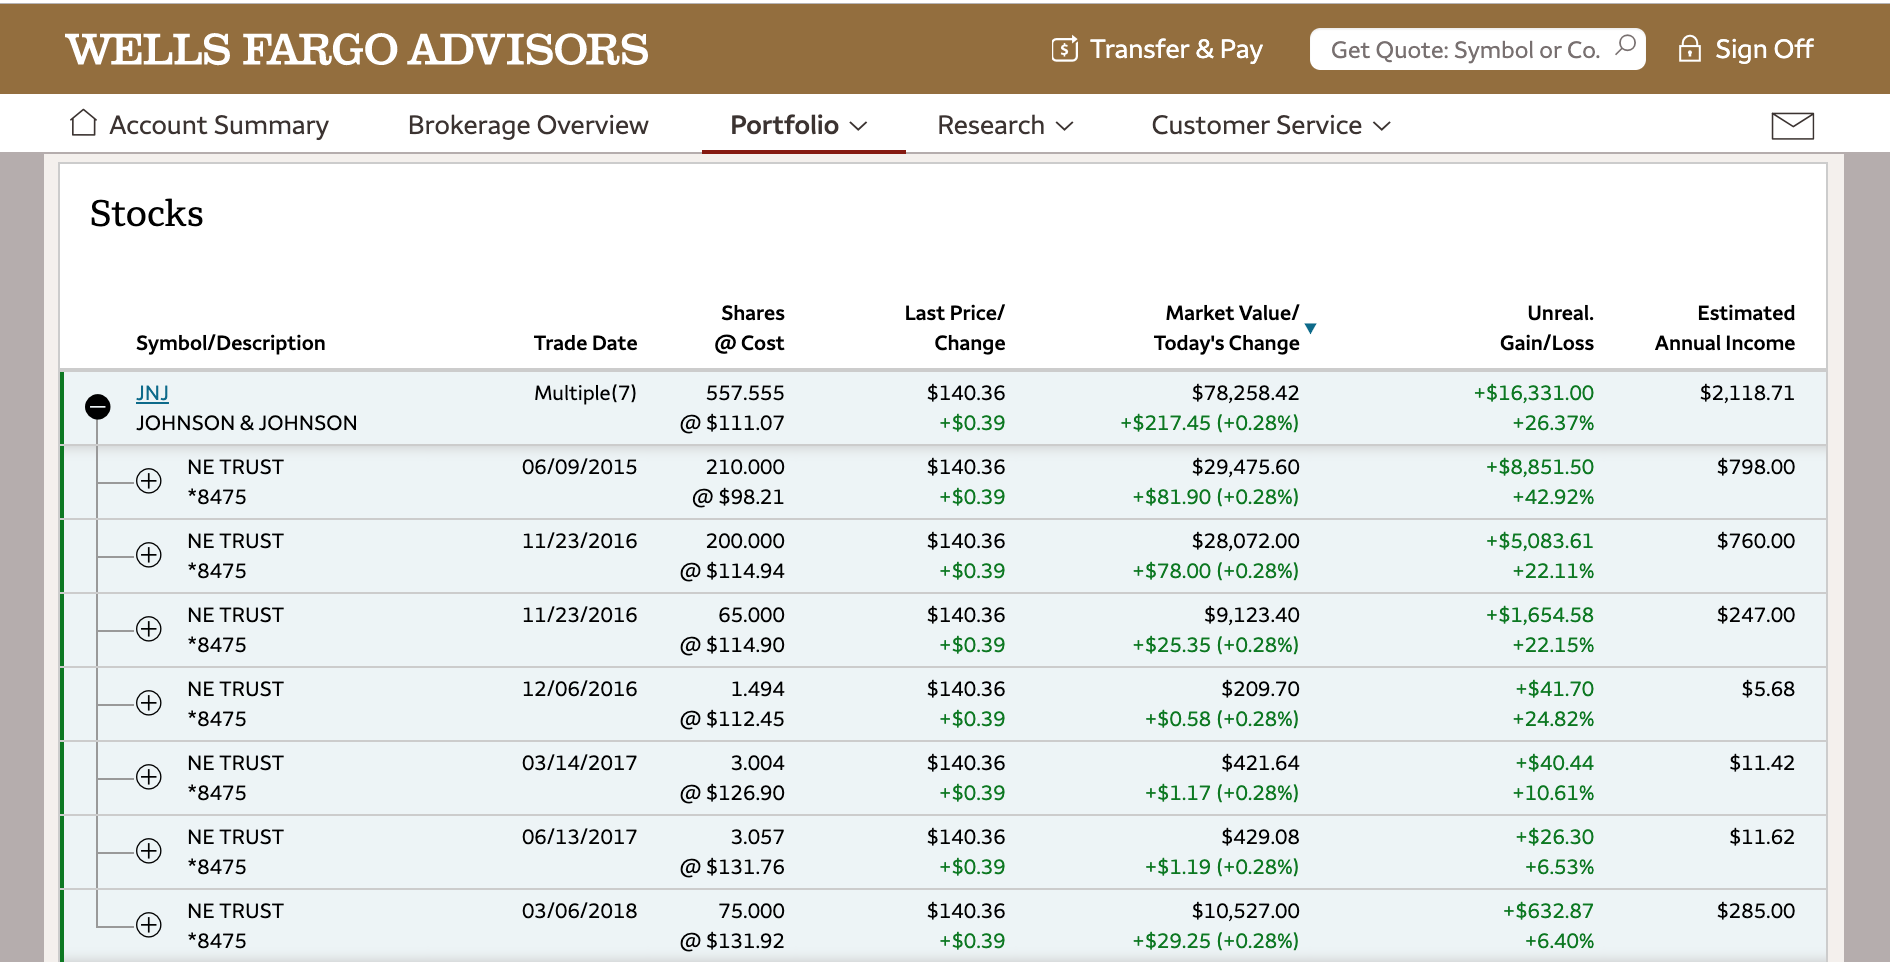
\includegraphics[scale=0.46] {images/jnj.png}}
\caption{JNJ numbers from Wells Fargo on 08-May-2019}
\label{fig:wfa}
\end{figure}

\bigskip
\noindent
\textbf{Example 2:}  For a more realistic example, suppose we want to take \$75,000.00 out of the Non-Exempt trust. One way this could be 
done is to sell part of the Non-Exempt trust's position in JNJ. These positions are shown in Figure \ref{fig:wfa}. Since JNJ is trading at  \$140.36,  
the trust needs to sell 75,000/140.36 = 534.35 or about 535 shares to generate \$75,000.00.

\bigskip
\noindent
Since we don't have 535 shares in any one JNJ position (see Figure \ref{fig:wfa}), we start by using the shares with the highest cost basis (in this case 131.92) and 
add up shares going from highest to lowest cost basis. Here we have


\begin{table}[H]
\centering
\begin{tabular}{c | c | c | c}
\text{\# shares} & \text{Cost Basis} & \text{Capital Gains/share} & \text{Total Capital Gains} \\
\hline
75.00  & 131.92 & 140.36 - 131.92 = 8.44    & 75.00 * 8.44     = 633.00 \\
3.057  & 131.76 & 140.36 - 131.76 = 8.60    & 3.057 * 8.60     = \: 26.29 \\
3.004  & 126.90 & 140.36 - 126.90 = 13.46  & 3.004 * 13.46 = 40.44 \\
1.494  & 112.45  & 140.36 - 112.45 = 27.91  & 1.494 * 27.91 = 41.70 \\
65.00  & 114.90  & 140.36 - 114.90 = 25.46  &  65.00 * 25.46 = 1654.90 \\
200.00 & 114.94 & 140.36 -114.94 = 25.42   & 200.00 * 25.42 = 5084.00 \\
187.45 & 98.21   & 140.36 - 98.21 = 42.15    & 187.45 * 42.15 = 7901.02 \\
\hline
\hline
535.005 &&& 15381.35
\end{tabular}
\caption{JNJ Positions: Cost Basis and Capital Gains}
\label{tab:jnj}
\end{table}




\bigskip
\noindent
As shown in Table \ref{tab:jnj}, the trust's capital gains on the sale of 535.005 shares of JNJ is  \$15,381.35 so the trust will incur 
capital gains tax of \$3,076.27 ($15381.35 *0.20 = 3076.27$), see Figure \ref{fig:2019_capital_gains_schedule}).
The total proceeds from the sale are $535.005 * \$140.36  = \$75,093.30$ (ignoring fees, etc).

\bigskip
\noindent
So if correct the trust could distribute $\$75,093.30 - \$3,076.27 = \$72,017.03$  to the beneficiary \textbf{tax-free}. 
BTW, this is an effective tax rate of  $(75093.30-72017.03)/75093.30 = .041$ or 4.1\%.



\section{Open Questions}
\label{sec:open_questions}

\begin{question}
Is the principal in the Exempt trust assumed to have been already taxed (like the Non-Exempt trust)? 
\end{question}

\begin{question}
Are there any restrictions on the distribution of principal, and if so is it different for the Exempt trust vs. the Non-Exempt Trust?
\end{question}

\begin{question}
Was the cost basis on the assets in the Wells Fargo trusts reset when we received the trusts? This one has no bearing on any of the above; just curiosity.
\end{question}


\bibliographystyle{plain}
\bibliography{/Users/dmm/papers/bib/family}
\end{document} 
